% ***************************************************
% A Classic Thesis Style
% An Homage to The Elements of Typographic Style
%
% Copyright (C) 2012 Andr\'e Miede http://www.miede.de
%
% If you like the style then I would appreciate a postcard. My
% address can be found in the file ClassicThesis.pdf. A collection
% of the postcards I received so far is available online at 
% http://postcards.miede.de
%
% License:
% This program is free software; you can redistribute it and/or
% modify it under the terms of the GNU General Public License as
% published by the Free Software Foundation; either version 2 of
% the License, or (at your option) any later version.
%
% This program is distributed in the hope that it will be useful,
% but WITHOUT ANY WARRANTY; without even the implied warranty of
% MERCHANTABILITY or FITNESS FOR A PARTICULAR PURPOSE.  See the
% GNU General Public License for more details.
%
% You should have received a copy of the GNU General Public
% License along with this program; see the file COPYING.  If not,
% write to the Free Software Foundation, Inc., 59 Temple Place -
% Suite 330, Boston, MA 02111-1307, USA.
%
% ***************************************************************
% Note:
%    * You must not use "u etc. in strings/commands that will be
%      spaced out (use \"u or real umlauts instead)
%    * New enumeration (small caps): \begin{aenumerate}
%      \end{aenumerate}
% 	 * For margin notes: \marginpar or \graffito{}
%    * Do not use bold fonts in this style, it is designed around
%      them
%    * Use tables as in the examples
%    * See classicthesis-preamble.sty for useful commands
% ****************************************************************

\documentclass[ twoside, 
				openright,
				% letterpaper a4paper
				titlepage, 
				numbers=noenddot,
				headinclude, %1headlines
				footinclude=true, 
				cleardoublepage=empty,
				%abstractoff, % <--- obsolete, remove (todo)
				BCOR=5mm,
				paper=a4, 
				fontsize=11pt, %11pt,
				]{scrreprt}

%*****************************************************************
% Note: Make all your adjustments in here
%*****************************************************************

\usepackage[backref, backend=biber]{biblatex}
\bibliography{Bibliography}	

% ****************************************************************
% classicthesis-config.tex 
% formerly known as loadpackages.sty, classicthesis-ldpkg.sty, and
% classicthesis-preamble.sty Use it at the beginning of your
% ClassicThesis.tex, or as a LaTeX Preamble in your
% ClassicThesis.{tex,lyx} with % ****************************************************************
% classicthesis-config.tex 
% formerly known as loadpackages.sty, classicthesis-ldpkg.sty, and
% classicthesis-preamble.sty Use it at the beginning of your
% ClassicThesis.tex, or as a LaTeX Preamble in your
% ClassicThesis.{tex,lyx} with % ****************************************************************
% classicthesis-config.tex 
% formerly known as loadpackages.sty, classicthesis-ldpkg.sty, and
% classicthesis-preamble.sty Use it at the beginning of your
% ClassicThesis.tex, or as a LaTeX Preamble in your
% ClassicThesis.{tex,lyx} with \input{classicthesis-config}
% ****************************************************************
% If you like the classicthesis, then I would appreciate a
% postcard. My address can be found in the file
% ClassicThesis.pdf. A collection of the postcards I received so
% far is available online at http://postcards.miede.de
% ****************************************************************

% ****************************************************************
% 1. Configure classicthesis for your needs here, e.g., remove
% "drafting" below in order to deactivate the time-stamp on the
% pages
% ****************************************************************
\PassOptionsToPackage{eulerchapternumbers,
						listings,
						%drafting,
						pdfspacing,
						floatperchapter,
						%linedheaders,
						subfig,
						beramono,
						eulermath,
						parts}{classicthesis}										

% ****************************************************************
% Triggers for this config
% **************************************************************** 
\usepackage{ifthen}
\newboolean{enable-backrefs} % enable backrefs in the bibliography
\setboolean{enable-backrefs}{false} % true false
% TODO backref is incompatible?
% ****************************************************************


% ****************************************************************
% 2. Personal data and user ad-hoc commands
% ****************************************************************
\newcommand{\myTitleIT}{Bluetooth Low Energy e Risparmio Energetico \xspace}
\newcommand{\myFirstAuthorName}{Lorenzo Pagliari\xspace}
\newcommand{\myMatrFirstAuthor}{798273\xspace}
\newcommand{\mySupervisor}{Prof.Raffaela Mirandola\xspace} % relatore
\newcommand{\myOtherSupervisor}{Diego Carmelo Perez Palacin\xspace} % co relatori
%\newcommand{\myFaculty}{Facolt\`a di Ingegneria\xspace}
\newcommand{\mySchool}{Scuola di Ingegneria Industriale e dell'Informazione\xspace}
\newcommand{\myDepartment}{Dipartimento di Elettronica, Informazione e Bioingegneria\xspace}
\newcommand{\myCourseFirstPartIT}{Corso di Laurea Magistrale in\xspace}
\newcommand{\myCourseSecondPartIT}{Ingegneria Informatica\xspace}
\newcommand{\myUni}{Politecnico di Milano\xspace}
\newcommand{\myLocation}{Milano\xspace}
\newcommand{\myTime}{Settembre 2015\xspace}
\newcommand{\myVersion}{version 1.0\xspace}
\newcommand{\myAcademicYear}{Anno Accademico 2014-2015\xspace}

% ********************************************************************
% Setup, fine tuning, and useful commands
% ********************************************************************
\newcounter{dummy} % necessary for correct hyperlinks (to index, bib, etc.)
\newlength{\abcd} % for ab..z string length calculation
\providecommand{\mLyX}{L\kern-.1667em\lower.25em\hbox{Y}\kern-.125emX\@}
% from here till the end of the section, you can modify whatever you want
\newcommand{\ie}{i.\,e.\ }
\newcommand{\Ie}{I.\,e.\ }
\newcommand{\eg}{e.\,g.\ }
\newcommand{\Eg}{E.\,g.\ }
% referencing commands
\newcommand{\myEq}[1]{equazione \eqref{#1}}
\newcommand{\MyEq}[1]{Equazione \eqref{#1}}
\newcommand{\myFig}[1]{figura \ref{#1}}
\newcommand{\MyFig}[1]{Figura \ref{#1}}
\newcommand{\myTab}[1]{tabella \ref{#1}}
\newcommand{\MyTab}[1]{Tabella \ref{#1}}
\newcommand{\mySubsec}[1]{sottosezione\ref{#1}}
\newcommand{\MySubsec}[1]{Sottosezione \ref{#1}}
\newcommand{\mySec}[1]{sezione \ref{#1}}
\newcommand{\MySec}[1]{Sezione \ref{#1}}
\newcommand{\myChap}[1]{capitolo \ref{#1}}
\newcommand{\MyChap}[1]{Capitolo \ref{#1}}
\newcommand{\myAppendix}[1]{appendice \ref{#1}}
\newcommand{\MyAppendix}[1]{Appendice \ref{#1}}
\newcommand{\myEmph}[1]{\textsc{#1}}

% **********************************************************************


% **********************************************************************
% 3. Loading some handy packages
% **********************************************************************
\PassOptionsToPackage{T1}{fontenc} % T2A for cyrillics
\usepackage{fontenc} 
\PassOptionsToPackage{utf8}{inputenc} % latin9 (ISO-8859-9) = latin1+"Euro sign"
\usepackage{inputenc}				

\PassOptionsToPackage{autostyle,italian=guillemets,threshold=2}{csquotes}
\usepackage{csquotes}

\PassOptionsToPackage{american,italian}{babel}
\usepackage{babel}

\PassOptionsToPackage{fleqn}{amsmath} % math environments and more by the AMS 
\usepackage{amsmath}

\usepackage{amsthm}
\theoremstyle{definition}

\newtheorem{definition}{Definition}

\usepackage{textcomp} % fix warning with missing font shapes
\usepackage{scrhack} % fix warnings when using KOMA with listings package          
\usepackage{xspace} % to get the spacing after macros right  
\usepackage{mparhack} % get marginpar right
\usepackage{fixltx2e} % fixes some LaTeX stuff 

\PassOptionsToPackage{printonlyused,smaller}{acronym}
\usepackage{acronym} % nice macros for handling all acronyms in the thesis
% **********************************************************************


% **********************************************************************
% 4. Setup floats: tables, (sub)figures, and captions
% **********************************************************************
\usepackage{tabularx} % better tables
\setlength{\extrarowheight}{3pt} % increase table row height
\newcommand{\tableheadline}[2]{\multicolumn{1}{#1}{\normalsize\spacedlowsmallcaps{#2}}}
\newcommand{\tableheadlineMore}[3]{\multicolumn{#1}{#2}{\normalsize\spacedlowsmallcaps{#3}}}
\newcommand{\tablefirstcol}[2]{\multicolumn{1}{#1}{\textbf{#2}}}

\usepackage{caption}
\captionsetup{format=hang,labelfont={sf,bf},font=small}
\usepackage{colortbl}
\usepackage{multirow}

\usepackage{subfig}
\usepackage{siunitx}
% *********************************************************************


% *********************************************************************
% 5. Setup code listings
% *********************************************************************
\usepackage{listings}
\lstloadlanguages{bash, C++, Java, Matlab}

% for special keywords
\lstset{language=[LaTeX]Tex,
	keywordstyle=\color{RoyalBlue},%\bfseries,
	basicstyle=\small\ttfamily,
	%identifierstyle=\color{NavyBlue},
	commentstyle=\color{Green}\ttfamily,
	stringstyle=\rmfamily,
	numbers=none,%left,%
	numberstyle=\scriptsize,%\tiny
	stepnumber=5,
	numbersep=8pt,
	showstringspaces=false,
	breaklines=true,
	frameround=ftff,
	frame=single,
	belowcaptionskip=.75\baselineskip
	%frame=L
} 
% *********************************************************************


% *********************************************************************
% 6. PDFLaTeX, hyperreferences and citation backreferences
% *********************************************************************
% ********************************************************************
% Using PDFLaTeX
% ********************************************************************
\PassOptionsToPackage{pdftex,hyperfootnotes=false,pdfpagelabels}{hyperref}
\usepackage{hyperref}  % backref linktocpage pagebackref
\pdfcompresslevel=9
\pdfadjustspacing=1 
\PassOptionsToPackage{pdftex}{graphicx}
\usepackage{graphicx} 

% ********************************************************************
% Setup the style of the backrefs from the bibliography
% (translate the options to any language you use)
% ********************************************************************
\newcommand{\backrefnotcitedstring}{\relax}%(Not cited.)
\newcommand{\backrefcitedsinglestring}[1]{(Cited on page~#1.)}
\newcommand{\backrefcitedmultistring}[1]{(Cited on pages~#1.)}
\ifthenelse{\boolean{enable-backrefs}}%
{%
	\PassOptionsToPackage{hyperpageref}{backref}
	\usepackage{backref} % to be loaded after hyperref package 
	\renewcommand{\backreftwosep}{ and~} % separate 2 pages
	\renewcommand{\backreflastsep}{, and~} % separate last of longer list
	\renewcommand*{\backref}[1]{}  % disable standard
	\renewcommand*{\backrefalt}[4]{% detailed backref
		\ifcase #1 %
		\backrefnotcitedstring%
		\or%
		\backrefcitedsinglestring{#2}%
		\else%
		\backrefcitedmultistring{#2}%
		\fi}%
}{\relax}    


% ****************************************************************
% PDF/A compliance
% ****************************************************************
% TODO not working: requires downloading color specification file in a specific
% tex folder and other hacks I don't want to spend time with
% \usepackage[a-1b]{pdfx}

% ********************************************************************
% Hyperreferences
% ********************************************************************
\hypersetup{%
	%draft,	% = no hyperlinking at all (useful in b/w printouts)
	colorlinks=true, linktocpage=true, pdfstartpage=3, pdfstartview=FitV,%
	% uncomment the following line if you want to have black links (e.g., for printing)
	%colorlinks=false, linktocpage=false, pdfborder={0 0 0}, pdfstartpage=3, pdfstartview=FitV,% 
	breaklinks=true, pdfpagemode=UseNone, pageanchor=true, pdfpagemode=UseOutlines,%
	plainpages=false, bookmarksnumbered, bookmarksopen=true, bookmarksopenlevel=1,%
	hypertexnames=true, pdfhighlight=/O,%nesting=true,%frenchlinks,%
	urlcolor=webbrown, linkcolor=RoyalBlue, citecolor=webgreen, %pagecolor=RoyalBlue,%
	%urlcolor=Black, linkcolor=Black, citecolor=Black, %pagecolor=Black,%
} 

%pdftitle={\myTitle},%
%pdfauthor={\textcopyright\ \myFirstAuthorName and \mySecondAuthorName, \myUni, \myFaculty},%
%pdfsubject={},%
%pdfkeywords={},%
%pdfcreator={pdfLaTeX},%
%pdfproducer={LaTeX with hyperref and classicthesis}%

%}   

% ********************************************************************
% Setup autoreferences
% ********************************************************************
% There are some issues regarding autorefnames
% http://www.ureader.de/msg/136221647.aspx
% http://www.tex.ac.uk/cgi-bin/texfaq2html?label=latexwords
% you have to redefine the makros for the 
% language you use, e.g., american, ngerman
% (as chosen when loading babel/AtBeginDocument)
% ********************************************************************
\makeatletter
\@ifpackageloaded{babel}%
{%
	\addto\extrasamerican{%
		\renewcommand*{\figureautorefname}{Figure}%
		\renewcommand*{\tableautorefname}{Table}%
		\renewcommand*{\partautorefname}{Part}%
		\renewcommand*{\chapterautorefname}{Chapter}%
		\renewcommand*{\sectionautorefname}{Section}%
		\renewcommand*{\subsectionautorefname}{Section}%
		\renewcommand*{\subsubsectionautorefname}{Section}% 	
	}%
	\addto\extrasitalian{% 
		\renewcommand*{\paragraphautorefname}{Paragrafo}%
		\renewcommand*{\subparagraphautorefname}{Paragrafo}%
		\renewcommand*{\footnoteautorefname}{Nota a pié di pagina}%
		\renewcommand*{\FancyVerbLineautorefname}{Zeile}%
		\renewcommand*{\theoremautorefname}{Teorema}%
		\renewcommand*{\appendixautorefname}{Appendice}%
		\renewcommand*{\equationautorefname}{Equazione}%        
		\renewcommand*{\itemautorefname}{Punto}%
	}%	
	% Fix to getting autorefs for subfigures right (thanks to Belinda Vogt for changing the definition)
	\providecommand{\subfigureautorefname}{\figureautorefname}%  			
}{\relax}
\makeatother

% ****************************************************************
% 7. Last calls before the bar closes
% ****************************************************************

\usepackage{classicthesis} 

% ****************************************************************
% ****************************************************************
% If you like the classicthesis, then I would appreciate a
% postcard. My address can be found in the file
% ClassicThesis.pdf. A collection of the postcards I received so
% far is available online at http://postcards.miede.de
% ****************************************************************

% ****************************************************************
% 1. Configure classicthesis for your needs here, e.g., remove
% "drafting" below in order to deactivate the time-stamp on the
% pages
% ****************************************************************
\PassOptionsToPackage{eulerchapternumbers,
						listings,
						%drafting,
						pdfspacing,
						floatperchapter,
						%linedheaders,
						subfig,
						beramono,
						eulermath,
						parts}{classicthesis}										

% ****************************************************************
% Triggers for this config
% **************************************************************** 
\usepackage{ifthen}
\newboolean{enable-backrefs} % enable backrefs in the bibliography
\setboolean{enable-backrefs}{false} % true false
% TODO backref is incompatible?
% ****************************************************************


% ****************************************************************
% 2. Personal data and user ad-hoc commands
% ****************************************************************
\newcommand{\myTitleIT}{Bluetooth Low Energy e Risparmio Energetico \xspace}
\newcommand{\myFirstAuthorName}{Lorenzo Pagliari\xspace}
\newcommand{\myMatrFirstAuthor}{798273\xspace}
\newcommand{\mySupervisor}{Prof.Raffaela Mirandola\xspace} % relatore
\newcommand{\myOtherSupervisor}{Diego Carmelo Perez Palacin\xspace} % co relatori
%\newcommand{\myFaculty}{Facolt\`a di Ingegneria\xspace}
\newcommand{\mySchool}{Scuola di Ingegneria Industriale e dell'Informazione\xspace}
\newcommand{\myDepartment}{Dipartimento di Elettronica, Informazione e Bioingegneria\xspace}
\newcommand{\myCourseFirstPartIT}{Corso di Laurea Magistrale in\xspace}
\newcommand{\myCourseSecondPartIT}{Ingegneria Informatica\xspace}
\newcommand{\myUni}{Politecnico di Milano\xspace}
\newcommand{\myLocation}{Milano\xspace}
\newcommand{\myTime}{Settembre 2015\xspace}
\newcommand{\myVersion}{version 1.0\xspace}
\newcommand{\myAcademicYear}{Anno Accademico 2014-2015\xspace}

% ********************************************************************
% Setup, fine tuning, and useful commands
% ********************************************************************
\newcounter{dummy} % necessary for correct hyperlinks (to index, bib, etc.)
\newlength{\abcd} % for ab..z string length calculation
\providecommand{\mLyX}{L\kern-.1667em\lower.25em\hbox{Y}\kern-.125emX\@}
% from here till the end of the section, you can modify whatever you want
\newcommand{\ie}{i.\,e.\ }
\newcommand{\Ie}{I.\,e.\ }
\newcommand{\eg}{e.\,g.\ }
\newcommand{\Eg}{E.\,g.\ }
% referencing commands
\newcommand{\myEq}[1]{equazione \eqref{#1}}
\newcommand{\MyEq}[1]{Equazione \eqref{#1}}
\newcommand{\myFig}[1]{figura \ref{#1}}
\newcommand{\MyFig}[1]{Figura \ref{#1}}
\newcommand{\myTab}[1]{tabella \ref{#1}}
\newcommand{\MyTab}[1]{Tabella \ref{#1}}
\newcommand{\mySubsec}[1]{sottosezione\ref{#1}}
\newcommand{\MySubsec}[1]{Sottosezione \ref{#1}}
\newcommand{\mySec}[1]{sezione \ref{#1}}
\newcommand{\MySec}[1]{Sezione \ref{#1}}
\newcommand{\myChap}[1]{capitolo \ref{#1}}
\newcommand{\MyChap}[1]{Capitolo \ref{#1}}
\newcommand{\myAppendix}[1]{appendice \ref{#1}}
\newcommand{\MyAppendix}[1]{Appendice \ref{#1}}
\newcommand{\myEmph}[1]{\textsc{#1}}

% **********************************************************************


% **********************************************************************
% 3. Loading some handy packages
% **********************************************************************
\PassOptionsToPackage{T1}{fontenc} % T2A for cyrillics
\usepackage{fontenc} 
\PassOptionsToPackage{utf8}{inputenc} % latin9 (ISO-8859-9) = latin1+"Euro sign"
\usepackage{inputenc}				

\PassOptionsToPackage{autostyle,italian=guillemets,threshold=2}{csquotes}
\usepackage{csquotes}

\PassOptionsToPackage{american,italian}{babel}
\usepackage{babel}

\PassOptionsToPackage{fleqn}{amsmath} % math environments and more by the AMS 
\usepackage{amsmath}

\usepackage{amsthm}
\theoremstyle{definition}

\newtheorem{definition}{Definition}

\usepackage{textcomp} % fix warning with missing font shapes
\usepackage{scrhack} % fix warnings when using KOMA with listings package          
\usepackage{xspace} % to get the spacing after macros right  
\usepackage{mparhack} % get marginpar right
\usepackage{fixltx2e} % fixes some LaTeX stuff 

\PassOptionsToPackage{printonlyused,smaller}{acronym}
\usepackage{acronym} % nice macros for handling all acronyms in the thesis
% **********************************************************************


% **********************************************************************
% 4. Setup floats: tables, (sub)figures, and captions
% **********************************************************************
\usepackage{tabularx} % better tables
\setlength{\extrarowheight}{3pt} % increase table row height
\newcommand{\tableheadline}[2]{\multicolumn{1}{#1}{\normalsize\spacedlowsmallcaps{#2}}}
\newcommand{\tableheadlineMore}[3]{\multicolumn{#1}{#2}{\normalsize\spacedlowsmallcaps{#3}}}
\newcommand{\tablefirstcol}[2]{\multicolumn{1}{#1}{\textbf{#2}}}

\usepackage{caption}
\captionsetup{format=hang,labelfont={sf,bf},font=small}
\usepackage{colortbl}
\usepackage{multirow}

\usepackage{subfig}
\usepackage{siunitx}
% *********************************************************************


% *********************************************************************
% 5. Setup code listings
% *********************************************************************
\usepackage{listings}
\lstloadlanguages{bash, C++, Java, Matlab}

% for special keywords
\lstset{language=[LaTeX]Tex,
	keywordstyle=\color{RoyalBlue},%\bfseries,
	basicstyle=\small\ttfamily,
	%identifierstyle=\color{NavyBlue},
	commentstyle=\color{Green}\ttfamily,
	stringstyle=\rmfamily,
	numbers=none,%left,%
	numberstyle=\scriptsize,%\tiny
	stepnumber=5,
	numbersep=8pt,
	showstringspaces=false,
	breaklines=true,
	frameround=ftff,
	frame=single,
	belowcaptionskip=.75\baselineskip
	%frame=L
} 
% *********************************************************************


% *********************************************************************
% 6. PDFLaTeX, hyperreferences and citation backreferences
% *********************************************************************
% ********************************************************************
% Using PDFLaTeX
% ********************************************************************
\PassOptionsToPackage{pdftex,hyperfootnotes=false,pdfpagelabels}{hyperref}
\usepackage{hyperref}  % backref linktocpage pagebackref
\pdfcompresslevel=9
\pdfadjustspacing=1 
\PassOptionsToPackage{pdftex}{graphicx}
\usepackage{graphicx} 

% ********************************************************************
% Setup the style of the backrefs from the bibliography
% (translate the options to any language you use)
% ********************************************************************
\newcommand{\backrefnotcitedstring}{\relax}%(Not cited.)
\newcommand{\backrefcitedsinglestring}[1]{(Cited on page~#1.)}
\newcommand{\backrefcitedmultistring}[1]{(Cited on pages~#1.)}
\ifthenelse{\boolean{enable-backrefs}}%
{%
	\PassOptionsToPackage{hyperpageref}{backref}
	\usepackage{backref} % to be loaded after hyperref package 
	\renewcommand{\backreftwosep}{ and~} % separate 2 pages
	\renewcommand{\backreflastsep}{, and~} % separate last of longer list
	\renewcommand*{\backref}[1]{}  % disable standard
	\renewcommand*{\backrefalt}[4]{% detailed backref
		\ifcase #1 %
		\backrefnotcitedstring%
		\or%
		\backrefcitedsinglestring{#2}%
		\else%
		\backrefcitedmultistring{#2}%
		\fi}%
}{\relax}    


% ****************************************************************
% PDF/A compliance
% ****************************************************************
% TODO not working: requires downloading color specification file in a specific
% tex folder and other hacks I don't want to spend time with
% \usepackage[a-1b]{pdfx}

% ********************************************************************
% Hyperreferences
% ********************************************************************
\hypersetup{%
	%draft,	% = no hyperlinking at all (useful in b/w printouts)
	colorlinks=true, linktocpage=true, pdfstartpage=3, pdfstartview=FitV,%
	% uncomment the following line if you want to have black links (e.g., for printing)
	%colorlinks=false, linktocpage=false, pdfborder={0 0 0}, pdfstartpage=3, pdfstartview=FitV,% 
	breaklinks=true, pdfpagemode=UseNone, pageanchor=true, pdfpagemode=UseOutlines,%
	plainpages=false, bookmarksnumbered, bookmarksopen=true, bookmarksopenlevel=1,%
	hypertexnames=true, pdfhighlight=/O,%nesting=true,%frenchlinks,%
	urlcolor=webbrown, linkcolor=RoyalBlue, citecolor=webgreen, %pagecolor=RoyalBlue,%
	%urlcolor=Black, linkcolor=Black, citecolor=Black, %pagecolor=Black,%
} 

%pdftitle={\myTitle},%
%pdfauthor={\textcopyright\ \myFirstAuthorName and \mySecondAuthorName, \myUni, \myFaculty},%
%pdfsubject={},%
%pdfkeywords={},%
%pdfcreator={pdfLaTeX},%
%pdfproducer={LaTeX with hyperref and classicthesis}%

%}   

% ********************************************************************
% Setup autoreferences
% ********************************************************************
% There are some issues regarding autorefnames
% http://www.ureader.de/msg/136221647.aspx
% http://www.tex.ac.uk/cgi-bin/texfaq2html?label=latexwords
% you have to redefine the makros for the 
% language you use, e.g., american, ngerman
% (as chosen when loading babel/AtBeginDocument)
% ********************************************************************
\makeatletter
\@ifpackageloaded{babel}%
{%
	\addto\extrasamerican{%
		\renewcommand*{\figureautorefname}{Figure}%
		\renewcommand*{\tableautorefname}{Table}%
		\renewcommand*{\partautorefname}{Part}%
		\renewcommand*{\chapterautorefname}{Chapter}%
		\renewcommand*{\sectionautorefname}{Section}%
		\renewcommand*{\subsectionautorefname}{Section}%
		\renewcommand*{\subsubsectionautorefname}{Section}% 	
	}%
	\addto\extrasitalian{% 
		\renewcommand*{\paragraphautorefname}{Paragrafo}%
		\renewcommand*{\subparagraphautorefname}{Paragrafo}%
		\renewcommand*{\footnoteautorefname}{Nota a pié di pagina}%
		\renewcommand*{\FancyVerbLineautorefname}{Zeile}%
		\renewcommand*{\theoremautorefname}{Teorema}%
		\renewcommand*{\appendixautorefname}{Appendice}%
		\renewcommand*{\equationautorefname}{Equazione}%        
		\renewcommand*{\itemautorefname}{Punto}%
	}%	
	% Fix to getting autorefs for subfigures right (thanks to Belinda Vogt for changing the definition)
	\providecommand{\subfigureautorefname}{\figureautorefname}%  			
}{\relax}
\makeatother

% ****************************************************************
% 7. Last calls before the bar closes
% ****************************************************************

\usepackage{classicthesis} 

% ****************************************************************
% ****************************************************************
% If you like the classicthesis, then I would appreciate a
% postcard. My address can be found in the file
% ClassicThesis.pdf. A collection of the postcards I received so
% far is available online at http://postcards.miede.de
% ****************************************************************

% ****************************************************************
% 1. Configure classicthesis for your needs here, e.g., remove
% "drafting" below in order to deactivate the time-stamp on the
% pages
% ****************************************************************
\PassOptionsToPackage{eulerchapternumbers,
						listings,
						%drafting,
						pdfspacing,
						floatperchapter,
						%linedheaders,
						subfig,
						beramono,
						eulermath,
						parts}{classicthesis}										

% ****************************************************************
% Triggers for this config
% **************************************************************** 
\usepackage{ifthen}
\newboolean{enable-backrefs} % enable backrefs in the bibliography
\setboolean{enable-backrefs}{false} % true false
% TODO backref is incompatible?
% ****************************************************************


% ****************************************************************
% 2. Personal data and user ad-hoc commands
% ****************************************************************
\newcommand{\myTitleIT}{Bluetooth Low Energy e Risparmio Energetico \xspace}
\newcommand{\myFirstAuthorName}{Lorenzo Pagliari\xspace}
\newcommand{\myMatrFirstAuthor}{798273\xspace}
\newcommand{\mySupervisor}{Prof.Raffaela Mirandola\xspace} % relatore
\newcommand{\myOtherSupervisor}{Diego Carmelo Perez Palacin\xspace} % co relatori
%\newcommand{\myFaculty}{Facolt\`a di Ingegneria\xspace}
\newcommand{\mySchool}{Scuola di Ingegneria Industriale e dell'Informazione\xspace}
\newcommand{\myDepartment}{Dipartimento di Elettronica, Informazione e Bioingegneria\xspace}
\newcommand{\myCourseFirstPartIT}{Corso di Laurea Magistrale in\xspace}
\newcommand{\myCourseSecondPartIT}{Ingegneria Informatica\xspace}
\newcommand{\myUni}{Politecnico di Milano\xspace}
\newcommand{\myLocation}{Milano\xspace}
\newcommand{\myTime}{Settembre 2015\xspace}
\newcommand{\myVersion}{version 1.0\xspace}
\newcommand{\myAcademicYear}{Anno Accademico 2014-2015\xspace}

% ********************************************************************
% Setup, fine tuning, and useful commands
% ********************************************************************
\newcounter{dummy} % necessary for correct hyperlinks (to index, bib, etc.)
\newlength{\abcd} % for ab..z string length calculation
\providecommand{\mLyX}{L\kern-.1667em\lower.25em\hbox{Y}\kern-.125emX\@}
% from here till the end of the section, you can modify whatever you want
\newcommand{\ie}{i.\,e.\ }
\newcommand{\Ie}{I.\,e.\ }
\newcommand{\eg}{e.\,g.\ }
\newcommand{\Eg}{E.\,g.\ }
% referencing commands
\newcommand{\myEq}[1]{equazione \eqref{#1}}
\newcommand{\MyEq}[1]{Equazione \eqref{#1}}
\newcommand{\myFig}[1]{figura \ref{#1}}
\newcommand{\MyFig}[1]{Figura \ref{#1}}
\newcommand{\myTab}[1]{tabella \ref{#1}}
\newcommand{\MyTab}[1]{Tabella \ref{#1}}
\newcommand{\mySubsec}[1]{sottosezione\ref{#1}}
\newcommand{\MySubsec}[1]{Sottosezione \ref{#1}}
\newcommand{\mySec}[1]{sezione \ref{#1}}
\newcommand{\MySec}[1]{Sezione \ref{#1}}
\newcommand{\myChap}[1]{capitolo \ref{#1}}
\newcommand{\MyChap}[1]{Capitolo \ref{#1}}
\newcommand{\myAppendix}[1]{appendice \ref{#1}}
\newcommand{\MyAppendix}[1]{Appendice \ref{#1}}
\newcommand{\myEmph}[1]{\textsc{#1}}

% **********************************************************************


% **********************************************************************
% 3. Loading some handy packages
% **********************************************************************
\PassOptionsToPackage{T1}{fontenc} % T2A for cyrillics
\usepackage{fontenc} 
\PassOptionsToPackage{utf8}{inputenc} % latin9 (ISO-8859-9) = latin1+"Euro sign"
\usepackage{inputenc}				

\PassOptionsToPackage{autostyle,italian=guillemets,threshold=2}{csquotes}
\usepackage{csquotes}

\PassOptionsToPackage{american,italian}{babel}
\usepackage{babel}

\PassOptionsToPackage{fleqn}{amsmath} % math environments and more by the AMS 
\usepackage{amsmath}

\usepackage{amsthm}
\theoremstyle{definition}

\newtheorem{definition}{Definition}

\usepackage{textcomp} % fix warning with missing font shapes
\usepackage{scrhack} % fix warnings when using KOMA with listings package          
\usepackage{xspace} % to get the spacing after macros right  
\usepackage{mparhack} % get marginpar right
\usepackage{fixltx2e} % fixes some LaTeX stuff 

\PassOptionsToPackage{printonlyused,smaller}{acronym}
\usepackage{acronym} % nice macros for handling all acronyms in the thesis
% **********************************************************************


% **********************************************************************
% 4. Setup floats: tables, (sub)figures, and captions
% **********************************************************************
\usepackage{tabularx} % better tables
\setlength{\extrarowheight}{3pt} % increase table row height
\newcommand{\tableheadline}[2]{\multicolumn{1}{#1}{\normalsize\spacedlowsmallcaps{#2}}}
\newcommand{\tableheadlineMore}[3]{\multicolumn{#1}{#2}{\normalsize\spacedlowsmallcaps{#3}}}
\newcommand{\tablefirstcol}[2]{\multicolumn{1}{#1}{\textbf{#2}}}

\usepackage{caption}
\captionsetup{format=hang,labelfont={sf,bf},font=small}
\usepackage{colortbl}
\usepackage{multirow}

\usepackage{subfig}
\usepackage{siunitx}
% *********************************************************************


% *********************************************************************
% 5. Setup code listings
% *********************************************************************
\usepackage{listings}
\lstloadlanguages{bash, C++, Java, Matlab}

% for special keywords
\lstset{language=[LaTeX]Tex,
	keywordstyle=\color{RoyalBlue},%\bfseries,
	basicstyle=\small\ttfamily,
	%identifierstyle=\color{NavyBlue},
	commentstyle=\color{Green}\ttfamily,
	stringstyle=\rmfamily,
	numbers=none,%left,%
	numberstyle=\scriptsize,%\tiny
	stepnumber=5,
	numbersep=8pt,
	showstringspaces=false,
	breaklines=true,
	frameround=ftff,
	frame=single,
	belowcaptionskip=.75\baselineskip
	%frame=L
} 
% *********************************************************************


% *********************************************************************
% 6. PDFLaTeX, hyperreferences and citation backreferences
% *********************************************************************
% ********************************************************************
% Using PDFLaTeX
% ********************************************************************
\PassOptionsToPackage{pdftex,hyperfootnotes=false,pdfpagelabels}{hyperref}
\usepackage{hyperref}  % backref linktocpage pagebackref
\pdfcompresslevel=9
\pdfadjustspacing=1 
\PassOptionsToPackage{pdftex}{graphicx}
\usepackage{graphicx} 

% ********************************************************************
% Setup the style of the backrefs from the bibliography
% (translate the options to any language you use)
% ********************************************************************
\newcommand{\backrefnotcitedstring}{\relax}%(Not cited.)
\newcommand{\backrefcitedsinglestring}[1]{(Cited on page~#1.)}
\newcommand{\backrefcitedmultistring}[1]{(Cited on pages~#1.)}
\ifthenelse{\boolean{enable-backrefs}}%
{%
	\PassOptionsToPackage{hyperpageref}{backref}
	\usepackage{backref} % to be loaded after hyperref package 
	\renewcommand{\backreftwosep}{ and~} % separate 2 pages
	\renewcommand{\backreflastsep}{, and~} % separate last of longer list
	\renewcommand*{\backref}[1]{}  % disable standard
	\renewcommand*{\backrefalt}[4]{% detailed backref
		\ifcase #1 %
		\backrefnotcitedstring%
		\or%
		\backrefcitedsinglestring{#2}%
		\else%
		\backrefcitedmultistring{#2}%
		\fi}%
}{\relax}    


% ****************************************************************
% PDF/A compliance
% ****************************************************************
% TODO not working: requires downloading color specification file in a specific
% tex folder and other hacks I don't want to spend time with
% \usepackage[a-1b]{pdfx}

% ********************************************************************
% Hyperreferences
% ********************************************************************
\hypersetup{%
	%draft,	% = no hyperlinking at all (useful in b/w printouts)
	colorlinks=true, linktocpage=true, pdfstartpage=3, pdfstartview=FitV,%
	% uncomment the following line if you want to have black links (e.g., for printing)
	%colorlinks=false, linktocpage=false, pdfborder={0 0 0}, pdfstartpage=3, pdfstartview=FitV,% 
	breaklinks=true, pdfpagemode=UseNone, pageanchor=true, pdfpagemode=UseOutlines,%
	plainpages=false, bookmarksnumbered, bookmarksopen=true, bookmarksopenlevel=1,%
	hypertexnames=true, pdfhighlight=/O,%nesting=true,%frenchlinks,%
	urlcolor=webbrown, linkcolor=RoyalBlue, citecolor=webgreen, %pagecolor=RoyalBlue,%
	%urlcolor=Black, linkcolor=Black, citecolor=Black, %pagecolor=Black,%
} 

%pdftitle={\myTitle},%
%pdfauthor={\textcopyright\ \myFirstAuthorName and \mySecondAuthorName, \myUni, \myFaculty},%
%pdfsubject={},%
%pdfkeywords={},%
%pdfcreator={pdfLaTeX},%
%pdfproducer={LaTeX with hyperref and classicthesis}%

%}   

% ********************************************************************
% Setup autoreferences
% ********************************************************************
% There are some issues regarding autorefnames
% http://www.ureader.de/msg/136221647.aspx
% http://www.tex.ac.uk/cgi-bin/texfaq2html?label=latexwords
% you have to redefine the makros for the 
% language you use, e.g., american, ngerman
% (as chosen when loading babel/AtBeginDocument)
% ********************************************************************
\makeatletter
\@ifpackageloaded{babel}%
{%
	\addto\extrasamerican{%
		\renewcommand*{\figureautorefname}{Figure}%
		\renewcommand*{\tableautorefname}{Table}%
		\renewcommand*{\partautorefname}{Part}%
		\renewcommand*{\chapterautorefname}{Chapter}%
		\renewcommand*{\sectionautorefname}{Section}%
		\renewcommand*{\subsectionautorefname}{Section}%
		\renewcommand*{\subsubsectionautorefname}{Section}% 	
	}%
	\addto\extrasitalian{% 
		\renewcommand*{\paragraphautorefname}{Paragrafo}%
		\renewcommand*{\subparagraphautorefname}{Paragrafo}%
		\renewcommand*{\footnoteautorefname}{Nota a pié di pagina}%
		\renewcommand*{\FancyVerbLineautorefname}{Zeile}%
		\renewcommand*{\theoremautorefname}{Teorema}%
		\renewcommand*{\appendixautorefname}{Appendice}%
		\renewcommand*{\equationautorefname}{Equazione}%        
		\renewcommand*{\itemautorefname}{Punto}%
	}%	
	% Fix to getting autorefs for subfigures right (thanks to Belinda Vogt for changing the definition)
	\providecommand{\subfigureautorefname}{\figureautorefname}%  			
}{\relax}
\makeatother

% ****************************************************************
% 7. Last calls before the bar closes
% ****************************************************************

\usepackage{classicthesis} 

% ****************************************************************

%*****************************************************************
% Hyphenation
%*****************************************************************
\hyphenation{put-here-the-words-latex-cannot-hyphenate}

\begin{document}
	
	% initial, local settings
	\numberwithin{equation}{chapter}
	\frenchspacing
	\raggedbottom
	\selectlanguage{italian} % american/italian
	\pagenumbering{roman}
	\pagestyle{plain}
	
	%*************************************************************
	% Frontmatter
	%*************************************************************
	
	% Uncomment the following line to add the ''copertina'' to the pdf
	% %*******************************************************
%
%			COPERTINA
%
%
%*******************************************************
\begin{titlepage}
	% if you want the titlepage to be centered, uncomment and fine-tune the line below (KOMA classes environment)
	\begin{addmargin}[-1cm]{-3cm}
	\begin{center}
		%\large %nse si usa 11pt
		\spacedlowsmallcaps{\myUni} \\
		\bigskip\myFaculty \\
		\medskip\mySchool \\
		\medskip\myDepartment \\
		\bigskip\myCourseFirstPartIT \\
		\medskip\myCourseSecondPartIT \\  
		
		\hfill
		
		\vfill
		
		\begin{figure}[!h]
			\begin{addmargin}[-1cm]{-3cm}
				\centering
				\includegraphics[width=0.3\columnwidth]{\myLogo} % or \logo.eps on windows 
			\end{addmargin}
		\end{figure}
		
		\vfill
		
		\begingroup
		%\huge %se si usa 11pt
		\LARGE %se si usa 12pt
		\color{Maroon} \myTitleIT \\ \bigskip
		\endgroup
		
		\vfill
		
		\flushleft 
		%\normalsize{Relatore:}\\ %se si usa 11pt
		\small{Relatore:}\\ %se si usa 12pt
		\medskip\spacedlowsmallcaps{\mySupervisor}
		
		\flushleft
		%\normalsize{Correlatore:}\\ %se si usa 11pt
		\small{Correlatore:}\\ %se si usa 12pt
		\medskip\spacedlowsmallcaps{\myOtherSupervisor}\\
		%comment if there isn't any other supervisor
		%\flushleft
		%\normalsize{Correlatore Alta Scuola Politecnica:}\\
		%\medskip\spacedlowsmallcaps{\myOtherOtherSupervisor}\\
		
		\vfill  
		
		\flushright
		%\normalsize{Tesi di Laurea Magistrale di:}\\ %se si usa 11pt
		\small{Tesi di Laurea Magistrale di:}\\ %se si usa 12pt
		\medskip \spacedlowsmallcaps{\myFirstAuthorName}\\
		Matricola n. \myMatrFirstAuthor \\ 
		
		\vfill 
		
		\centering {\myAcademicYear}                     
		
	\end{center}
	\end{addmargin}
\end{titlepage}
	%%*******************************************************
% Titlepage
%   the file is named in italian since our language 
%   provide different words for different things and
%   we should use them
%*******************************************************
\begin{titlepage}
	% if you want the titlepage to be centered, uncomment and
	% fine-tune the line below (KOMA classes environment)
	% \begin{addmargin}[-1cm]{-3cm}
    \begin{center}
    	\large
        \spacedlowsmallcaps{\myUni} \\
        \bigskip\myFaculty \\
        %\medskip\mySchool \\
    	\medskip\myDepartment \\
    	\bigskip\myCourseFirstPart \\
        \medskip\myCourseSecondPart \\  

        \hfill

        \vfill
        
        \begin{figure}[!h]
			\begin{center}
				
\includegraphics[width=0.3\columnwidth]{Images/logoPoli.pdf} 
				% or \logo.eps on windows 
			\end{center}
		\end{figure}
		
		\vfill

        \begingroup
       		\huge	
            \color{Maroon} \myTitle
            \bigskip
        \endgroup

        \vfill

		\flushleft 
		\normalsize{Supervisor:}\\
		\medskip\spacedlowsmallcaps{\mySupervisor}

		\flushleft
		\normalsize{Assistant Supervisor:}\\
		\medskip\spacedlowsmallcaps{\myOtherSupervisor}\\
		%comment if there is another supervisor
		%\flushleft
		%\normalsize{Alta Scuola Politecnica Assistant Supervisors:}\\
		%\medskip\spacedlowsmallcaps{\myOtherOtherSupervisor}\\
        
        \vfill  
        
        \flushright
        \normalsize{Master Graduation Thesis by:}\\
        \medskip \spacedlowsmallcaps{\myFirstAuthorName}\\
		Student Id n. \myMatrFirstAuthor \\ 
		% uncomment if there is a second author
		%\medskip\spacedlowsmallcaps{\mySecondAuthorName} \\
		%Student Id n. \myMatrSecondAuthor \\
		
		\vfill 

		\centering {\myAcademicYear}                     

    \end{center}  
  %\end{addmargin}       
\end{titlepage}
	%*******************************************************
% Titlepage
%   the file is named in italian since our language 
%   provide different words for different things and
%   we should use them
%*******************************************************
\begin{titlepage}
	% if you want the titlepage to be centered, uncomment and fine-tune the line below (KOMA classes environment)
	% \begin{addmargin}[-1cm]{-3cm}
    \begin{center}
    	\large
        \spacedlowsmallcaps{\myUni} \\
        \bigskip
        %\myFaculty \\
        \medskip\mySchool \\
    	\medskip\myDepartment \\
    	\bigskip\myCourseFirstPartIT \\
        \medskip\myCourseSecondPartIT \\  

        \hfill

        \vfill
        
        \begin{figure}[!h]
			\begin{center}
				
\includegraphics[width=0.3\columnwidth]{Images/logoPoli.pdf} % or \logo.eps on windows 
			\end{center}
		\end{figure}
		
		\vfill

        \begingroup
       		\huge	
            \color{Maroon} \myTitleIT \\ \bigskip
        \endgroup

        \vfill

		\flushleft 
		\normalsize{Relatore:}\\
		\medskip\spacedlowsmallcaps{\mySupervisor}

		\flushleft
		\normalsize{Correlatore:}\\
		\medskip\spacedlowsmallcaps{\myOtherSupervisor}\\
		%comment if there isn't any other supervisor
		%\flushleft
		%\normalsize{Correlatore Alta Scuola Politecnica:}\\
		%\medskip\spacedlowsmallcaps{\myOtherOtherSupervisor}\\
        
        \vfill  
        
        \flushright
        \normalsize{Tesi di Laurea Magistrale di:}\\
        \medskip \spacedlowsmallcaps{\myFirstAuthorName}\\
		Matricola n. \myMatrFirstAuthor \\ 
				
		\vfill 

		\centering {\myAcademicYear}                     

    \end{center}  
  %\end{addmargin}       
\end{titlepage}
	%\thispagestyle{empty}

\hfill

\vfill

\pdfbookmark[0]{Colophon}{colophon}
\section*{Colophon}
This document was typeset using the typographical look-and-feel
\texttt{classicthesis} developed by Andr\'e Miede.
The style was inspired by Robert Bringhurst's seminal book on
typography ``\emph{The Elements of Typographic Style}''.
\texttt{classicthesis} is available for both \LaTeX\ and \mLyX: 
\begin{center}
\url{http://code.google.com/p/classicthesis/}
\end{center}
Happy users of \texttt{classicthesis} usually send a real postcard
to the author, a collection of postcards received so far is
featured here:
\begin{center}
\url{http://postcards.miede.de/}
\end{center}
 
\bigskip

\noindent\myFirstAuthorName:
\textit{\myTitleIT},
\myTime

\medskip

%\noindent\finalVersionString % a.k.a. the colophon
	\cleardoublepage%*******************************************************
% Dedication
%*******************************************************
\thispagestyle{empty}
%\phantomsection 
\stepcounter{dummy}
\pdfbookmark[1]{Dediche}{Dediche}

\vspace*{3cm}
\begin{center}
	DEDICHE \\ \medskip
	Dedico questo lavoro a ... \\
\end{center}
	% \cleardoublepage%*******************************************************
% Publications
%*******************************************************
\pdfbookmark[1]{Publications}{publications}
\chapter*{Publications}
Some ideas and figures have appeared previously in the following
publications:

\bigskip

\noindent Put your publications from the thesis here. The packages 
\texttt{multibib} or \texttt{bibtopic} etc. can be used to handle
multiple different bibliographies in your document.

	\cleardoublepage%*******************************************************
% Acknowledgments
%*******************************************************
\pdfbookmark[1]{Ringraziamenti}{Ringraziamenti}

\bigskip

\begingroup
\let\clearpage\relax
\let\cleardoublepage\relax
\let\cleardoublepage\relax
\chapter*{RINGRAZIAMENTI}
Ringrazierò qualcuno ahahah.... 

\endgroup
	\cleardoublepage%*******************************************************
% Table of Contents
%*******************************************************
%\phantomsection
\stepcounter{dummy}
\pdfbookmark[1]{\contentsname}{tableofcontents}
\setcounter{tocdepth}{2} % <-- 2 includes up to subsections in the ToC
\setcounter{secnumdepth}{3} % <-- 3 numbers up to subsubsections
%PER AVERE I DOTS nelle liste, bisogna aggiungere "dottedtoc" alle opzioni in \PassOptionsToPackage{...,dottedtoc}{classicthesis}
\manualmark
\markboth{\spacedlowsmallcaps{\contentsname}}{\spacedlowsmallcaps{\contentsname}}
\tableofcontents 
\automark[section]{chapter}
\renewcommand{\chaptermark}[1]{\markboth{\spacedlowsmallcaps{#1}}{\spacedlowsmallcaps{#1}}}
\renewcommand{\sectionmark}[1]{\markright{\thesection\enspace\spacedlowsmallcaps{#1}}}
%*******************************************************
% List of Figures and of the Tables
%*******************************************************
\clearpage

\begingroup 
    \let\clearpage\relax
    \let\cleardoublepage\relax
    \let\cleardoublepage\relax
    %*******************************************************
    % List of Figures
    %*******************************************************    
    %\phantomsection 
    \stepcounter{dummy}
    %\addcontentsline{toc}{chapter}{\listfigurename}
    \pdfbookmark[1]{\listfigurename}{lof}
    \listoffigures

    \vspace*{8ex}

    %*******************************************************
    % List of Tables
    %*******************************************************
    %\phantomsection 
    \stepcounter{dummy}
    %\addcontentsline{toc}{chapter}{\listtablename}
    \pdfbookmark[1]{\listtablename}{lot}
    \listoftables
        
    \vspace*{8ex}
%   \newpage
    
    %*******************************************************
    % List of Listings
    %*******************************************************      
	  %\phantomsection 
    \stepcounter{dummy}
    %\addcontentsline{toc}{chapter}{\lstlistlistingname}
    \pdfbookmark[1]{\lstlistlistingname}{lol}
    \lstlistoflistings 

    \vspace*{8ex}
       
    %*******************************************************
    % Acronyms
    %*******************************************************
    %\phantomsection 
    \stepcounter{dummy}
    \pdfbookmark[1]{Acronimi}{Acronimi}
    \markboth{\spacedlowsmallcaps{Acronyms}}{\spacedlowsmallcaps{Acronyms}}
    \chapter*{Acronimi}
	    % environment acronym take the longest acronym as parameter to
    % determine the wideness of columns. Put it between square bracket
    \begin{acronym}[XML]
    	% put here the acronyms you use and recall them in text by
    	% using \ac{NAME}. In the text you can also use \acs{}, \acf{}, \acl{}
    	% for various flavours
    	\acro{OS}{Operating System}
    	\acro{XML}{eXtensible Markup Language}
    	%*************************************%
    	\acro{IT}{Information Technology}
    	\acro{QoS}{qualità del servizio}
    	\acro{DVS}{Dynamic frequency/voltage scaling}
    	\acro{ACPI}{Advanced Configuration and Power Interface}
    	\acro{BT}{Bluetooth}
    	\acro{BLE}{Bluetooth Low Energy}
    	\acro{PB}{Probabilistic Broadcast}
    	\acro{PE}{Probabilistic Edge}
    	\acro{FF}{Fixed Fanout}
    	\acro{DF}{Dyanmic Fanout}
    	\acro{AL}{Advertising Limit}
    	\acro{AE}{Advertising Event}
    	\acro{CE}{Connection Event}
    	\acro{P2P}{Peer-to-Peer}
    	\acro{RGG}{Random Geometric Graph}
    	\acro{SI}{Suscettible – Infected}
    	\acro{SIS}{Suscettible – Infected – Suscettible}
    	\acro{SIR}{Suscettible – Infected – Removed}
    	\acro{LTE}{Long Term Evolution}
    	\acro{MCC}{Mobile Cloud Computing}
    	\acro{NED}{Network Definition}
    \end{acronym}                  
\endgroup

\cleardoublepage
	\cleardoublepage%*******************************************************
% Abstract
%*******************************************************
%\renewcommand{\abstractname}{Abstract}
\addcontentsline{toc}{chapter}{\abstractname}

\pdfbookmark[1]{Sommario}{Sommario}
\begingroup
\let\clearpage\relax
\let\cleardoublepage\relax
\let\cleardoublepage\relax

\chapter*{Sommario}
Questo lavoro si posiziona nell'ambito del risparmio energetico e nell'ambito delle applicazioni per dispositivi mobili. Abbiamo studiato una possibile soluzione in grado di trasmettere informazioni attraverso dispositivi mobili, quando si verificano scenari nei quali le comuni reti di telecomunicazione non sono disponibili. Scenari di questo tipo possono essere causati facilmente da forti e avverse condizioni meteorologiche. Grossi nubifragi, forti nevicate o altri eventi di questo genere, possono facilmente danneggiare la struttura della rete di telecomunicazioni, causando l'inattività delle stesse. La nostra idea è stata di progettare un sistema in grado di sfruttare i comuni dispositivi elettronici più diffusi e, tramite le tecnologie a disposizione, trovare un modo alternativo per diffondere le informazioni tra le persone. Lavorando con dispositivi mobili, e' stato necessario considerare le problematiche collegate al consumo energetico. Uno degli obiettivi del sistema che presenteremo in questo elaborato, è quello di regolare il carico di lavoro che si vuole assegnare al dispositivo, in modo da trovare sempre un compromesso tra prestazioni e autonomia residua della batteria.
In questo elaborato presenteremo la soluzione da noi proposta, illustrando i principi degli algoritmi utilizzati per guidare la diffusione dell'informazione, i modelli usati per descrivere la rete di dispositivi mobili e la tecnologia di trasmissione utilizzata.
\endgroup
	%\cleardoublepage%*****************************************************************
% Breve riassunto in italiano della tesi da cui si capisca tutto
% ****************************************************************
\newcommand{\estrattoname}{Estratto}
\addcontentsline{toc}{chapter}{\estrattoname}

\pdfbookmark[1]{Estratto}{Estratto}
\begingroup
\let\clearpage\relax
\let\cleardoublepage\relax
\let\cleardoublepage\relax

\chapter*{Estratto}
\enquote{\ldots il testo delle tesi redatte in lingua straniera dovrà essere introdotto da un
ampio estratto in lingua italiana, che andrà collocato dopo l’abstract.}

\endgroup


	%\cleardoublepage
\addcontentsline{toc}{chapter}{\prefacename}
\pdfbookmark[1]{Preface}{Preface}

\chapter*{Preface}
A preface is an introduction to a book or other literary work
written by the work's author. A preface generally covers the story
of how the book came into being, or how the idea for the book was
developed.

\section*{Motivation}
Graduating is not the motivation that one expects here.

	
	\pagestyle{scrheadings}	
	
	%*************************************************************
	% Mainmatter
	
	%*************************************************************
	\pagenumbering{arabic}
	%\setcounter{page}{90}
	% use \cleardoublepage here in case of problems with pdfbookmark
	
	\cleardoublepage\ctparttext{You can put some informational part preamble text here.}
	\part{Writing a Master thesis}
	
	\chapter{An introduction to the writing of scientific texts}
\label{chap:aChapter}
\begin{flushright}{\slshape    
   Science, my boy, is made up of mistakes, but they are mistakes
   which it is useful to make, because they lead little by little
   to the truth}. \\ \medskip --- \citeauthor{verne_journey:1957}
   \citetitle{verne_journey:1957}
\end{flushright} 

\section{The structure of a scientific text}

\section{Bibliographies and literature reviews}

\section{A tentative index}

\section{Follow the instructions}
Visit \href{http://www.tedoc.polimi.it/tesilaurea/Consegna-tesi-di-laurea-(vecchio-ordinamento-e-specialistica)}{this link} for the updated information about the content of the thesis.

\enquote{Alcune Scuole forniscono linee guida specifiche cui i laureandi devono attenersi per la redazione della tesi. Per ulteriori informazioni:
\href{http://www.tedoc.polimi.it/download/lauree_magistrali/201406_POLITesi_Info_specifiche_scuole.pdf}{www.tedoc.polimi.it/\ldots}}

\subsection{Archiving electronic documents: PDF/A}
PDF/A is an ISO-standardized version of the Portable Document Format (PDF) specialized for the digital preservation of electronic documents. PDF/A differs from PDF by prohibiting features ill-suited to long-term archiving, such as font linking (as opposed to font embedding). The ISO requirements for PDF/A file viewers include color management guidelines, support for embedded fonts, and a user interface for reading embedded annotations.

Universities usually requires this standard but they're also not aware that common programs like MS Word, OpenOffice and so on aren't really able to produce compliant PDFs. In Latex, there's some development going on but at the time of writing, the available commands are still too obscure and buggy. So in the end, forget the PDF/A for now.\footnote{Or DIY and then make a pull request on github :D.}
	% \include{Chapter/MyOtherChapter}
	
	\cleardoublepage\ctparttext{Another informational part preamble text here.}
	\part{Using this Latex template}
	
	\chapter{Practical guide to \enquote{ClassicThesis at DEIB}}
\label{chap:conclusion}
This template is ready to be used when writing a thesis at \myDepartment.
It is a modified version of Classic Thesis by Andr\'e Miede that can be found here \url{http://code.google.com/p/classicthesis/}.

\section{Learn \LaTeX}
\LaTeX\ is a document preparation system and document markup language.
It is widely used for the communication and publication of scientific documents in many fields, including mathematics, physics, computer science, statistics, economics, and political science.

\LaTeX\ users are weird people who care about the ligature between \enquote{f} and \enquote{i} and gets pissed off every time they look at a MS Word document.
Nevertheless, they can explain themselves very well as shown in some beautiful guides for the \LaTeX\ world.
My preferred one for beginners is \enquote{The Not So Short Introduction to \LaTeXe}, which can be found \href{http://www.ctan.org/pkg/lshort}{here}.\footnote{\url{http://www.ctan.org/pkg/lshort}}
For italians I also strongly suggest \enquote{L'arte di scrivere con \LaTeX}, that can be found \href{http://www.lorenzopantieri.net/LaTeX_files/ArteLaTeX.pdf}{here}.\footnote{\url{http://www.lorenzopantieri.net/LaTeX_files/ArteLaTeX.pdf}}
It contains everything needed, however I suggest the reading of chapter 3 for a short introduction. \enquote{ClassicThesis} is another guide of the same author that can be useful, download it \href{http://www.lorenzopantieri.net/LaTeX_files/ClassicThesis.pdf}{here}.\footnote{\url{http://www.lorenzopantieri.net/LaTeX_files/ClassicThesis.pdf}}

\section{Install \LaTeX}
If you don't have already a \LaTeX\ system installed, this section will explain everything you need.
The easiest way to get \LaTeX\ is to install TeXLive, which works on all \acp{OS}.
In \url{https://www.tug.org/texlive/} you find the instructions and the files needed - and also get in touch with minimalism of \TeX users. 

Then you will need an editor: I strongly recommend TeXworks because it's very simple and available on all the platforms.
Also you don't need to install it, it's already included in TeXLive.
The official documentation of TeXworks is available \href{https://docs.google.com/file/d/0B5iVT8Q7W44pMk1WSFRKcDRlMU0/preview}{here};\footnote{\url{https://docs.google.com/file/d/0B5iVT8Q7W44pMk1WSFRKcDRlMU0/preview}}
I strongly recommend the reading of chapter 3.
Alternatevely you can read an italian manual: \href{http://profs.sci.univr.it/~gregorio/introtexworks.pdf}{profs.sci.univr.it/\ldots} (just 13 pages, read it!).\footnote{If you already have a preferred editor, just keep using yours.}

After opening TeXworks, I strongly suggest to set these two additional things:
\begin{itemize}
	\item open Preferences, then go the Composition tab: in the second box there, the \enquote{Process instruments}, push the plus button.
In the window just opened, write \verb!Biber! in the \enquote{Name} field, \verb!biber! in the \enquote{Program} field (lowercase!) and then press the plus button to add the argument \verb!$basename!;
	\item again in the same window, set \enquote{Hide console output} to \enquote{never}.
\end{itemize}

Then just test the installation of the template:
\begin{aenumerate}
	\item go into the template home folder;
	\item open the file \verb!ClassicThesis_DEIB.tex!;
	\item select \verb!pdfLaTeX! from the dropdown menu in the top right of the TeXworks window;
	\item press the rounded green button: it compiles the \verb!.tex! file for the first time and open the resulting \verb!.pdf!;
	\item select \verb!Biber! from the same dropdown menu and press again the green button: this compiles the bibliography, a thing you need to repeat only when you change the file \verb!Bibliography.bib!;
	\item select \verb!pdfLaTeX! again and recompile: this is needed to build indices and crossreferences;
\end{aenumerate}
The above compilation procedure is the standard way to translate the \LaTeX\ code into pdfs.

\section{Online editor}
If the above procedure seems too difficult to you and you have an internet connection always available, you might think to use an online editor. The best choice at the time of writing is \url{http:\\\\sharelatex.com} where you can even find this template after registration to the site by looking for \enquote{Classic Thesis At DEIB}. Your project will be saved on their server but you can also download them. The platform allows up to two authors for free accounts.

There is no need to provide instructions for its use since the website has them. They also have an online \LaTeX guide which is also very useful.

\section{Building blocks}

\subsection{File structure}
The template is organized in multiple file and folders:
\begin{aenumerate}

	\item \verb!ClassicThesis_DEIB.tex! is the main file to be compiled, found in the root folder.
You should just add the source filenames you want to include and any hyphenation you need to explictly specify. 

	\item \verb!classicthesis-config.tex! contains options that can be chosen for this template, like the \verb!draft! one that prints date and time at the bottom of every page.
It contains also the definition for the title, the author and others stuff displayed in the titlepage.
Comments within the file should guide you.\footnote{comments are the rows starting with $\%$.} Take a look at it!

	\item \verb!Bibliography.bib! is the \emph{Bibtex} database: it is a normal textfile where you should put books and articles read;

	\item \verb!Chapters! contains the files for the main chapters of your thesis; this is where you will add the chapters text, as well these very words in line 41 of the file \verb!Conclusion.tex!;

	\item \verb!CodeFiles! contains any code snippet you want to include in your thesis with the environment \verb!listings!; it might be some relevant Matlab or C code, as well as long bash scripts;

	\item \verb!FrontBackmatter! contains various files that are included in the main one to produce abstract, titlepages, acknowledgements, \ldots. 
Follow the instructions below to modify them in order to suits your needs;

	\item \verb!Images! contains the \verb!.pdf! or \verb!.png! versions of the images of the thesis.
A \verb!sources! subfolder is also provided for keeping things well organized.

\end{aenumerate}

To modify abstract, preface, acknowledgements snd acronyms, you need to go into the folder \verb!FrontBackmatter! where you will find the following:
\begin{description}

	\item[Abstract.tex] contains the text displayed as \enquote{abstract} and \enquote{sommario} just after the list of figures, tables, etc. Modify the text and leave the rest.

	\item[Acknowledgments.tex] contains the text put just before the table of contents. Modify the text to suit your needs.

	\item[Acronyms.tex] contains the environment \verb!acronym! with the definition of all the acronyms that will be used within the text. Add your own to the list and put the longest as parameter of the environment.
 
	\item[AutoParts] folder contains things that should work without your intervention. Forget them. 

	\item[Dedication.tex] same usage and structure as \verb!Acknowledgements.tex!.

	\item[Estratto.tex] Politecnico di Milano requires an italian long excerpt of theses written in foreign languages.

	\item[Frontespizio.tex] and \verb!FrontespizioIT.tex! are the cover page in english and italian, respectively. Politecnico di Milano requires the italian version of the english cover, so there it is. Both should work perfectly if you modify section 2 of the file \verb!classicthesis-config.tex!, but you may not like the style so modify them as you prefer.
	
	\item[Preface.tex] same usage and structure as \verb!Acknowledgements.tex!.

	\item[Publication.tex] same usage and structure as \verb!Acknowledgements.tex!, but not included by default. Activate it by uncommenting the relevant line in \verb!ClassicThesis_DEIB.tex!.

	\item[RetroFrontespizio.tex] contains the colophon. In most cases is fine as it already is.
\end{description}

\subsection{Environments}
In addition to common \LaTeX\ environments, this thesis is set to use:
\begin{itemize}

	\graffito{The command graffito is used to put some text here, usefull to underline important things before long paragraphs.}

	\item \verb!\begin{aenumerate}! to produce an \verb!\enumerate! with letters instead of numbers, as in the file list above;

	\item \verb!\blockcquote[][]{}{}! to 	\blockcquote[see][p. 111]{bringhurst:2002}{produce a citation
	with reference to author and page}. If the citation is longer than two rows is indented.
This is provided by the package \verb!csquotes!, which settings are in	\verb!classicthesis-config.tex!.
The package also provides \verb!\enquote{!the citation\verb!}! that produces \enquote{correct citation style} according to the language in use.

	\item \verb!\ac{}! and its variations, defined by package \verb!acronyms!, provide nice handling for acronyms, like \ac{XML}, produced with the code \verb!\ac{XML}!.
List them within the environment \verb!acronym! in the file \verb!FrontBackmatter/Acronyms.tex!.

	\item the so called semi-dynamic referencing for chapter, sections, subsections, appendices, figures, tables and equations. They are a set of commands like \verb!\myChap{label_key}! that produce things like \myChap{chap:aChapter}. There are also capital versions of the commands (\verb!\MyChap{}! produces \MyChap{chap:aChapter}). They need a \verb!\label{name}! anchor next to the referred thing.
	\begin{itemize}
		\item\verb!\myChap! for chapters;
		\item\verb!\mySec! for sections;
		\item\verb!\mySubsec! for subsections;
		\item\verb!\myAppendix! for appendices;
		\item\verb!\myFig! for figures;
		\item\verb!\myTab! for tables;
		\item\verb!\myEq! for equations;
	\end{itemize}

	\item references to bibliography are produced in the usual way with \verb!\cite{bib_key}! \cite{bringhurst:2002} and its variations \verb!\citeauthor{bib_key}!, \verb!\citetitle{bib_key}! and others.

	\item figures are handled usually with the code
	\begin{verbatim}
	\begin{figure}
	\centering
	\includegraphics[width=\columnwidth]{Images/your_image_name.pdf} 
	\caption[Short description]{Long description.}
	\label{fig:a_name}
	\end{figure}
	\end{verbatim}
	which produces things like \myFig{fig:massConstraintFeasibility}. Of course, you need to put the image file \verb!your_image_name.pdf! in folder \verb!Images/!.

	\item tables are produced with
	\begin{verbatim}
	\begin{table}[tb]
	\footnotesize
	\centering
	\begin{tabularx}{0.8\textwidth}{llrcl}
	\toprule
	\tableheadline{l}{Algorithm} &
	\tableheadline{l}{Parameter} &
	\tableheadlineMore{3}{c}{Suggested Values} \\
	\midrule
	\tablefirstcol{l}{Any}
	& \acs{NFE} 		& $10\,000 $ & $ \div $ & $ 200\,000$ \\
	& Population Size 	&  $10 $ & $ \div 	$ & $ 1000$ \\
	\midrule
	\tablefirstcol{l}{\ac{GDE3}}
	& \ac{DE} step size & $0.0 $ & $\div $ & $ 1.0$ \\
	& Crossover rate 	& $0.0$ & $ \div $ & $ 1.0$ \\
	\bottomrule
	\end{tabularx}
	\caption[Short description]{Long description.}
	\label{tab:MOEAandParameters}
	\end{table}
	\end{verbatim}
	which produces \myTab{tab:MOEAandParameters}.
\verb!\myfloatalign!, \verb!\tableheadline{}{}! and its variation \verb!\tableheadlineMore{}{}{}! and \verb!\tablefirstcol{}{}! are used to give a common style to all tables in the document.
They are defined in \verb!classicthesis-config.tex!.\footnote{Also do not forget footnotes, created by \texttt{\textbackslash footnote\{\}}, which should be placed after the punctuation mark.}

	\item equation are produced in classic \LaTeX\ way and they turn out be something like this
	\begin{equation}
	\nabla \mathbf{q_s} = U(x,y) - b_t
	\label{eq:massConservation}
	\end{equation}

\end{itemize}

\begin{figure}
\centering
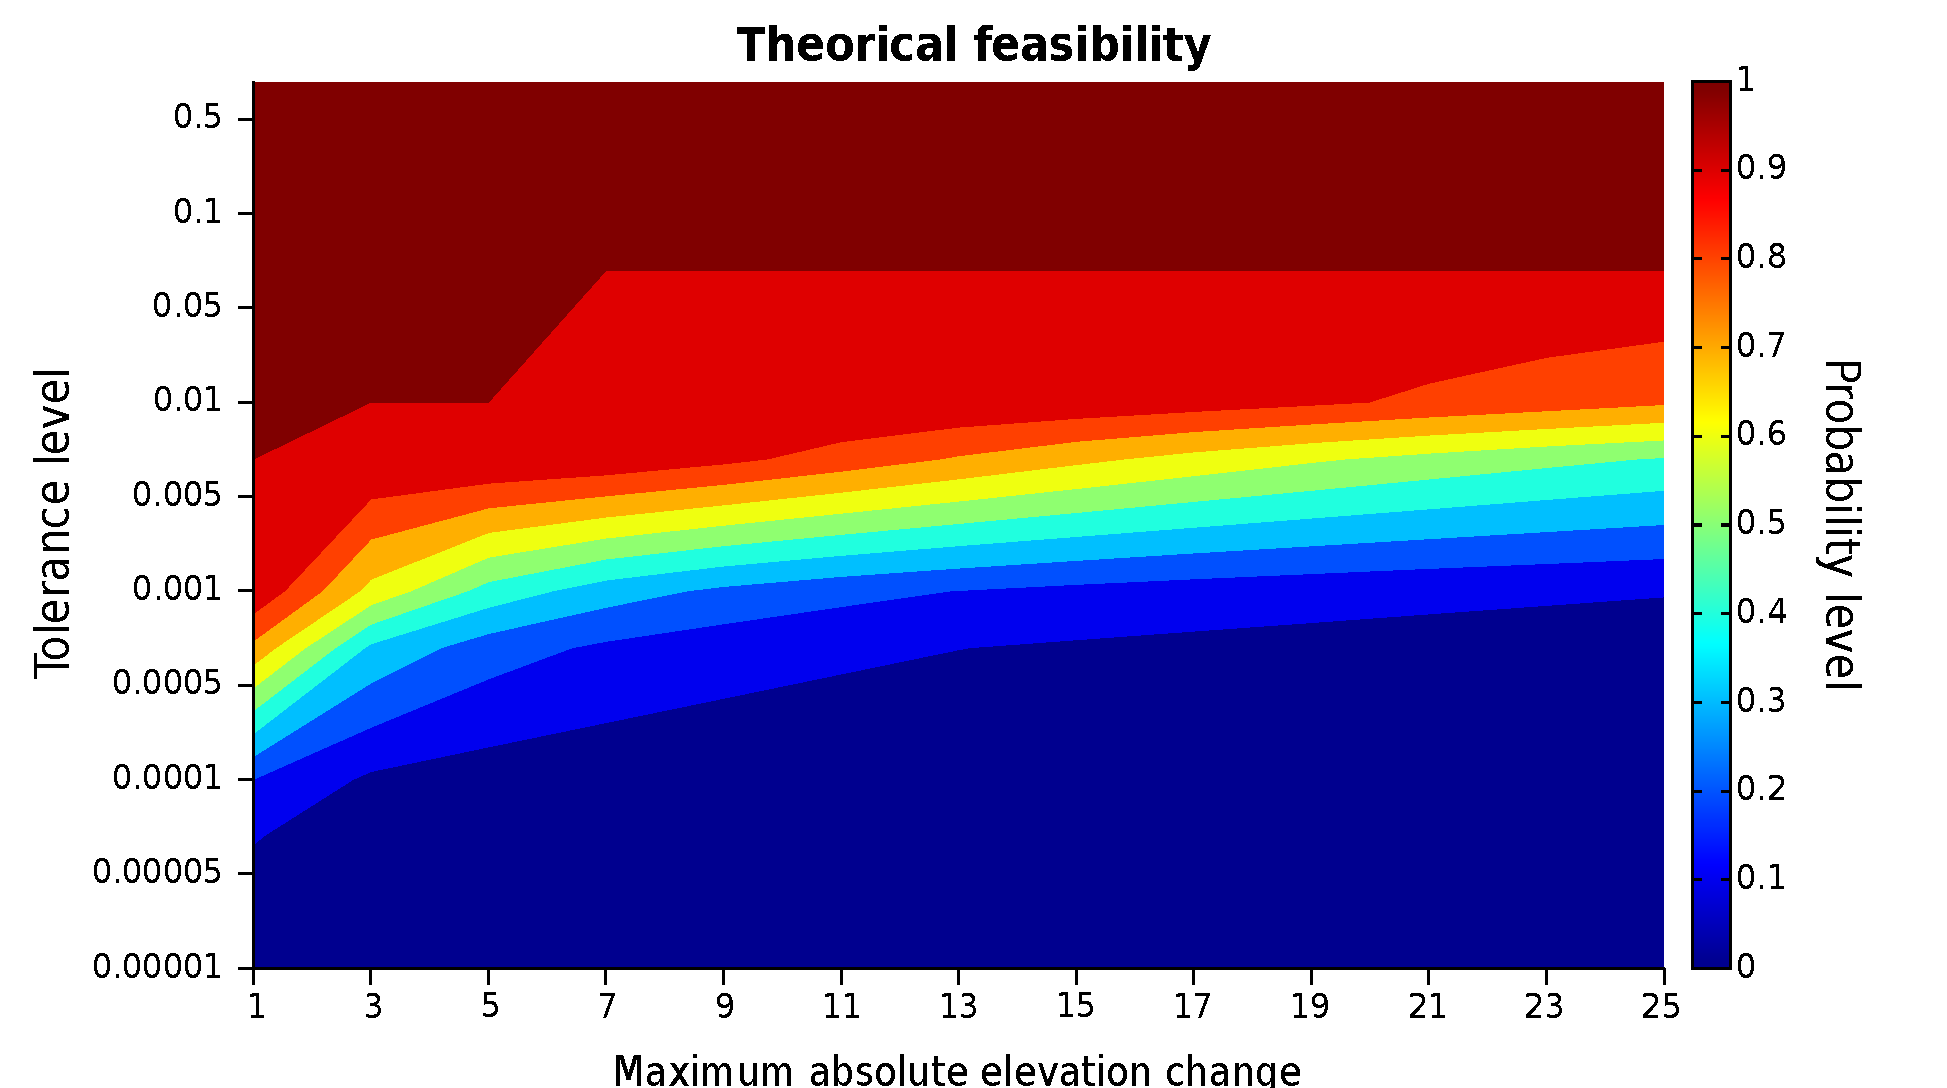
\includegraphics[width=\columnwidth]{Images/feasibilityNR51.pdf}  
\caption[Thing taken from our master thesis]{Thing taken from our master thesis whose meaning have been completely forgotten.}
\label{fig:massConstraintFeasibility}
\end{figure}

\begin{table}
\footnotesize
\centering
\begin{tabularx}{0.8\textwidth}{llrcl}
\toprule
\tableheadline{l}{Algorithm} &
\tableheadline{l}{Parameter} &
\tableheadlineMore{3}{c}{Suggested Values} \\
\midrule
\tablefirstcol{l}{Any}	& NFE	 		& $10\,000 $ 	& $ \div $ 	& $ 200\,000$ \\
				& Population Size 	&  $10 $ 		& $ \div $ 	& $ 1000$ \\
\midrule
\tablefirstcol{l}{GDE3} & DE step size 		& $0.0 $ 	& $\div $ 	& $ 1.0$ \\
				& Crossover rate 	& $0.0$ 	& $ \div $ 	& $ 1.0$ \\
\bottomrule
\end{tabularx}
\caption[Parameters needed for things]{Parameters needed for things that are not needed anymore themselves.}
\label{tab:MOEAandParameters}
\end{table}

\section{Contributing to this template}
Suggestion and improvements are welcome at \url{https://github.com/Lordmzn/ClassicThesis-at-DEIB} or via email at \url{emanuele.mason@polimi.it} or \url{andrea.cominola@polimi.it}.
 
	
	% ************************************************************
	% Backmatter
	%*************************************************************
	\cleardoublepage%********************************************************************
% Bibliography
%*******************************************************
% work-around to have small caps also here in the headline
\manualmark
\markboth{\spacedlowsmallcaps{\bibname}}{\spacedlowsmallcaps{\bibname}}
%\phantomsection 
\stepcounter{dummy} 
% to have the bib a bit from the rest in the toc
\addtocontents{toc}{\protect\vspace{\beforebibskip}}
\addcontentsline{toc}{chapter}{\tocEntry{\bibname}}
\label{app:bibliography}
\printbibliography
	\appendix
	\cleardoublepage\part{Appendix}
	%********************************************************************
% Appendix
%*******************************************************
% If problems with the headers: get headings in appendix etc. right
\markboth{\spacedlowsmallcaps{Appendix}}{\spacedlowsmallcaps{Appendix}}
%************************************************
\chapter{Appendix}

\section{Diagrammi di flusso algoritmo Dyanimc Fanout}
\subsection{Standby FSA}
\label{apx:stb_fsa}
\begin{figure}[h]
	\centering
	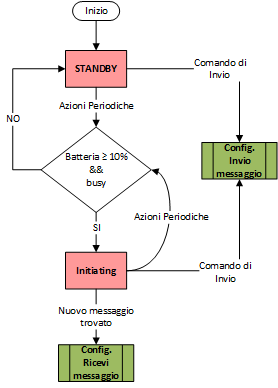
\includegraphics[]{Images/diagrammi_fsa/Standby_fsa}
	\caption[Standby fsa]{Diagramma di flusso della macchina a stati Standby.}
	\label{fig:Standby_fsa}
\end{figure}
\newpage

\subsection{Invia Messaggio FSA}
\label{apx:invio_fsa}
\begin{figure}[!h]
	\centering
	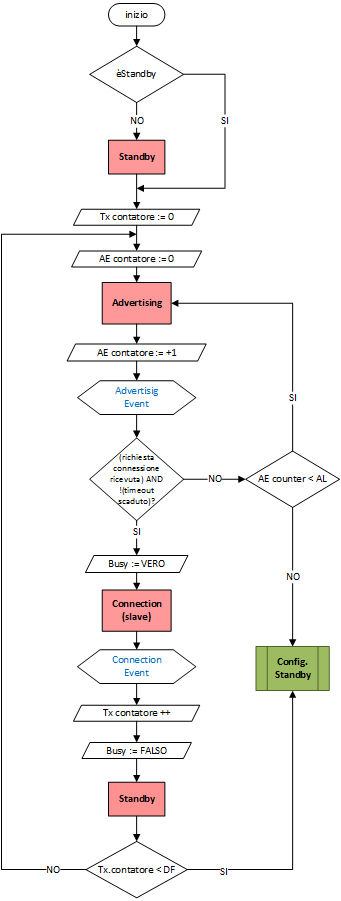
\includegraphics[height= 0.78\textheight]{Images/diagrammi_fsa/Invio_msg_fsa}
	\caption[Invio Messaggio fsa]{Diagramma di flusso della macchina a stati Invio Messaggio.}
	\label{fig:Invio_msg_fsa}
\end{figure}
\newpage
\subsection{Ricevi Messaggio FSA}
\label{apx:ricevi_fsa}
\begin{figure}[!h]
	\centering
	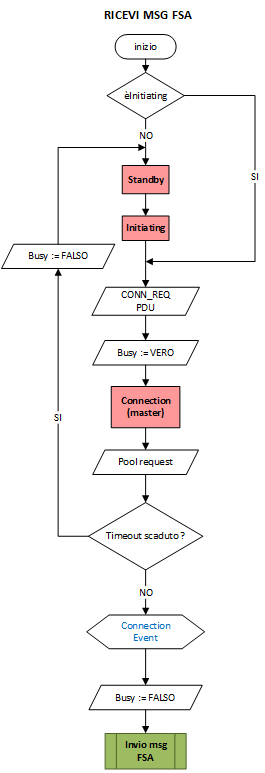
\includegraphics[height= 0.78\textheight]{Images/diagrammi_fsa/Ricevi_msg_fsa}
	\caption[Ricevi Messaggio fsa]{Diagramma di flusso della macchina a stati Ricevi Messaggio.}
	\label{fig:Ricevi_msg_fsa}
\end{figure}


	
\end{document}
% ****************************************************************